\documentclass[12pt]{beamer}
\usetheme{Madrid}
\usepackage[utf8x]{inputenc}
\usepackage{ucs}
\usepackage{amsmath}
\usepackage{amsfonts}
\usepackage{amssymb}
\usepackage{graphicx}
\author{CHARPIGNON Thibault \\ GALLET Benoît \\ HERRMMAN Emmanuel \\ RETY Martin \\}
\title{GraphoScan}
\institute{ Université d'Orléans \\ \medskip \textit{Encadré par : EXBRAYAT Matthieu} }

\begin{document}

\begin{frame}
\titlepage
\end{frame}


\begin{frame}
\frametitle{Introduction}
\framesubtitle{Paléographie}
\begin{definition}
Science de l'étude des écritures manuscrites anciennes
\end{definition}
\begin{block}{Composé de}
\begin{itemize}
\item Lecture et édition des textes
\item Étude des systèmes de production de l'écriture
\item Évolution des écritures dans le temps
	\begin{itemize}
	\item Ductus : ordre et sens du tracé de la lettre
	\end{itemize}
\end{itemize}
\end{block}
\end{frame}

\begin{frame}
\frametitle{Introduction}
\framesubtitle{Objectif et solution}
\begin{block}{Objectif de GraphoScan}
\begin{itemize}
\item Relation mouvement de la plume / trace écrite
\item Proposer une nouvelle représentation des écritures médiévales
\end{itemize}
\end{block}

\begin{block}{Solution}
\begin{itemize}
\item Structure en bois avec deux caméras
\item Application séparée en deux
	\begin{itemize}
	\item Acquisition de l'écriture
	\item Tracking et reconstruction 3D du mouvement
	\end{itemize}
\end{itemize}
\end{block}
\end{frame}


\begin{frame}
\frametitle{Plan}
\tableofcontents
\end{frame}

\section{Projet Originel}
\section{Travail Réalisé}
\section{Projet Final}
\section{Conclusion}

\begin{frame}
\Huge{\centerline{Projet Originel}}
\end{frame}

\begin{frame}
\frametitle{Projet Originel}
\framesubtitle{Travail Effectué}
\begin{itemize}
\item{C++ avec OpenGL, OpenCV et Matlab}
\item Structure :
\begin{figure}
\includegraphics[width=0.5\textwidth]{../Rapport/Modules/Picture/Utilisation.png}
\end{figure}
\end{itemize}
\end{frame}

\begin{frame}
\frametitle{Projet Originel}
\framesubtitle{Travail Effectué}
\begin{enumerate}
\item Acquisition vidéo
\begin{itemize}
\item Calibrage des caméras
\item Acquisition en stéréo
\item Correction de la distorsion pour lisser l'image
\end{itemize}
\item Tracking
\begin{itemize}
\item Région d'interêt (ROI)
\item Histogramme de gradient orienté (HOG)
\end{itemize}
\item Reconstruction 3D
\begin{itemize}
\item Calcul des points 3D avec OpenCV
\item Reconstruction 3D avec OpenGL
\end{itemize}
\end{enumerate}
\end{frame}

\begin{frame}
\frametitle{Projet Originel}
\framesubtitle{Problèmes}
\begin{itemize}
\item Fréquence d'acquisition trop faible (8 images par seconde)
\item Eclairage du dispositif trop faible entrainant des zones d'ombres
\item Déplacement du support d'écriture impossible
\item Gestes de relaxation de l'utilisateur non gérés
\item Code non nettoyé, non documenté et copié depuis internet
\end{itemize}
\end{frame}

\begin{frame}
\Huge{\centerline{Travail Réalisé}}
\end{frame}

\begin{frame}
\frametitle{Travail réalisé}
\framesubtitle{Organisation}
\begin{itemize}
\item Projet en deux parties
\item Groupe séparé en deux
	\begin{itemize}
	\item Acquisition : Emmanuel + Benoît
	\item Tracking et reconstruction : Martin + Thibault
	\end{itemize}
\end{itemize}
\end{frame}

\begin{frame}
\frametitle{Travail réalisé}
\framesubtitle{Travail effectué}
\begin{figure}
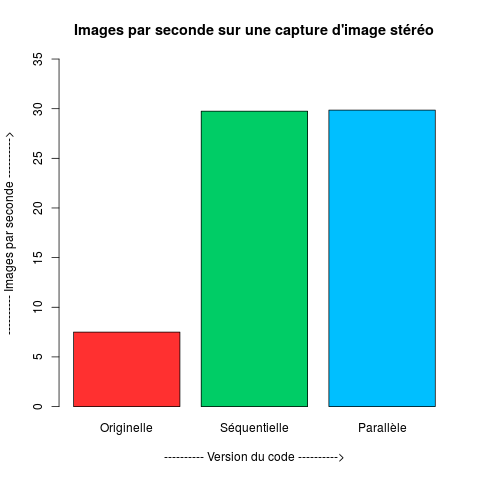
\includegraphics[width=0.5\textwidth]{../Rapport/Modules/Picture/fps.png}
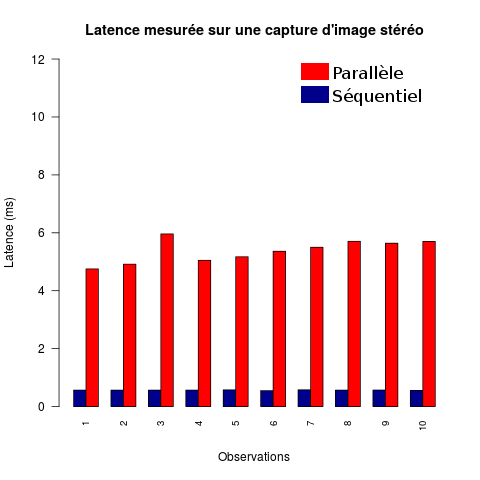
\includegraphics[width=0.5\textwidth]{../Rapport/Modules/Picture/latence.png}
\end{figure}
\end{frame}

\begin{frame}
\frametitle{Travail réalisé}
\framesubtitle{Travail effectué}
\begin{itemize}
\item Augmentation des FPS / diminution de la latence
\item Parallélisation
\item Généralisation à n caméras
\item Nettoyage du code
\item Choix de l'algorithme de tracking
\item Écriture des shaders
\end{itemize}
\end{frame}

\begin{frame}
\Huge{\centerline{Projet Final}}
\end{frame}

\begin{frame}
\frametitle{Projet Final}
\framesubtitle{Vidéo de présentation}
\begin{enumerate}
\item Choix des images
\item Sélection de la ROI
\item Application de l'algorithme de tracking
\item Affichage des résultats
\item Affichage de la reconstruction 3D
\end{enumerate}
\end{frame}

\begin{frame}
\frametitle{Projet Final}
\framesubtitle{Améliorations possibles}
\begin{itemize}
\item Droit d'auteur
\item Interface graphique
\item Amélioration du tracking
\begin{itemize}
\item Déplacement de la feuille
\item Mouvements parasites
\end{itemize}
\item Synchronisation native
\item Reconstruction 3D
\end{itemize}
\end{frame}

\begin{frame}
\frametitle{Conclusion}
\framesubtitle{Compétences}
\begin{itemize}
\item UE de Programmation parallèle
\item UE de Programmation graphique
\item UE d'Outils pour l'exploration de données
\item UE d'Analyse des algorithmes
\item Utilisation de MatLab
\item Utilisation d'algorithmes de tracking
\end{itemize}
\end{frame}

\begin{frame}
\frametitle{Conclusion}
\framesubtitle{Résumé}
\begin{itemize}
\item Avant : Projet peu performant et brouillon
\item Maintenant : Projet commenté, documenté, avec un manuel, toutes les parties fonctionnelles
\item Améliorations possibles
\item Des améliorations rendues simples à implémenter grâce au travail réalisé
\end{itemize}
\end{frame}

\begin{frame}
\Huge{\centerline{Merci pour votre attention}}
\end{frame}

\end{document}